\documentclass[11pt]{beamer}
\usepackage[utf8]{inputenc}
\usepackage[T1]{fontenc}
\usepackage{lmodern}
\usetheme{Rochester}
\usepackage{graphicx}
\begin{document}
	\title{\textbf{Website Design Ranker}}
	\subtitle{Using Machine Learning}
	%\logo{}
	\institute{\large Department of Computer Science and Engineering \\\textbf{FISAT}}
	\date{21 NOVEMBER 2019}
	\author{{\scriptsize Adhyaksh Guhan - 7 , Anet Eliza Johny - 23 , Dharwish Raj - 47 , \\ Joel J Padayattil - 60}}
	%\setbeamercovered{transparent}
	%\setbeamertemplate{navigation symbols}{}
	\begin{frame}[plain]
		\maketitle
	\end{frame}
	\begin{frame}{Problem Statement}
		\begin{itemize}
			
			
			\item Our project is aimed at ranking websites in terms of its design which is evaluated baised on certain parameters.
			
			\item Since a perfect model for website ranking  is not in practice, this follows ranking according to submissions by critics.
			
			\item Our main problem is to evaluate website designs using an algorithm.As there was no algorithms or methods existing to rank website design.
			
	
			
		\end{itemize}
	\end{frame}
	\begin{frame}{Related Works}
		\begin{itemize}
			
		\section{Google Page Layout Algorithm}
		Google introduced Page Layout Algorithm to analyze website
		readability.[1] It looks for the layout of the web page and the amount of
		content we see in the page once we click on a result.[1] It focuses to reduce the difficulty of users to find the actual
		content.[1]
		The websites which does not have a lot of visible content
		above-the-fold and dedicates a large fraction (above a normal
		degree) to ads, will be affected.[1]
		\begin{figure}
			
			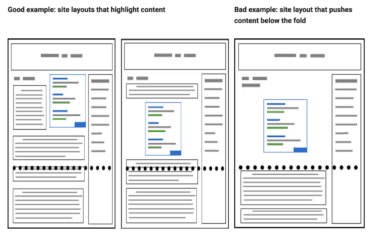
\includegraphics[width=10cm]{image/gpa.png}
			\caption{One of the criteria of GPL Algorithm\textsuperscript{[Fig:1]}}
			\label{fig1:gpa}
			
		\end{figure}
		
		
		Determine the old design of the website.If a website has many advertisements above the fold(the part of page that is visible on the screen when the page first loads before scrolling)then it is considered as the first drawback.Else if a website has a large flash animations or other
		non-content elements that forces users to scroll to see the content, then that will be the next drawback. If there is specific amount of ads and content of website required for audience, there will be no drawback.These drawbacks will affect the ranking process. If these conditions are met the website ranks a low rank. Else its rank will be considerabily high.
		
		
			
	
			
		\end{itemize}
	\end{frame}
	\begin{frame}{Proposed System}
			\begin{itemize}
			\item Website Design Ranker will rank set of input websites based on certain parameters.
			\item The parameters we are focussing on are color and grid .
			\item Then we move on for public review.
			\item This will be helpful to finding the best website among list of websites.
			\item We can compare our website design with other competing websites.
			\item We can see how a website's design may improve in an area.

			\end{itemize}
	\end{frame}
	\begin{frame}{Explanation }
		\begin{itemize}
			\item It is an objective analysis of website designs by ranking them based on a parameter.
			\item The website's CSS file is scrapped via a web scrapper and then read through.
			\item The file is then parsed to find hex codes based on a regular expression.
			\item Once the codes are found, they are counted and printed using a variable.
		\end{itemize}
	\end{frame}
		\begin{frame}{Methodology used}
	\begin{itemize}
		\item Using the basis of colour theory, we count the number of colours to determine the ranking of the website.
		\item Too few colours, then the website is extremely simple and too boring.
		\item Too many colours, then the website is over-designed and busy. 
	\end{itemize}
	\end{frame}
	\begin{frame}
	\frametitle{{Algorithm}}
	\begin{enumerate}
	\item Start
	\item Using a website scraper to accept the various website addresses
	\item Scraping through the source code of each website via CSS files
	\item Find the hex codes of all elements of the website and count them with a count variable
	\item If count == 0
	\item [(4.1)] Give mark as 0
	\item else if count > 5
	\item [(5.1)] Give mark as 0
	\item else if count <= 5
	\item [(6.1)] Give mark as 1
	\item Stop
	\end{enumerate}
	
	\end{frame}
	\begin{frame}
	\frametitle{{Current Status}}
		\begin{itemize}
		\item The website for public ranking of website designs is 90 percent complete.
		\item Main colour code segment is working and needs to be unified under one file.
	\end{itemize}
	\end{frame}
\begin{frame}
			\frametitle{{Project Completion Time}}
	\begin{itemize}
		\item 22nd November, 2019
	\end{itemize}
\end{frame}

\begin{frame}{Experimental result}
			\begin{itemize}
				\item An example 'style.css' from a website template was downloaded and parsed through to test the colour code program. The number of colour codes were found and printed.
				\item A number of websites' front page's screenshots were taken using the website screenshot program. 
			\end{itemize}	
	\end{frame}

	\begin{frame}{Social and ethical relevance}
		\begin{itemize}
			\item Eliminates subjectivity and unfair competitions based on peoples' biases.
			\item Shows how to improve user experience of a website by showing the problems of the website.
		\end{itemize}
	\end{frame}

	\begin{frame}{Conclusion}
		\begin{itemize}
			\item Here we can see the logical differences in the approaches that our algorithm takes versus any existing methods.
			\item Our method relies on an objective and automated method that is consistent in nature as opposed to the subjective methods of the existing methods.
		\end{itemize}
	\end{frame}
\end{document}
